\documentclass[12pt, a4paper, titlepage, final]{article}


\usepackage[utf8]{inputenc}
\usepackage[british]{babel}
\usepackage[T1]{fontenc}
\usepackage{graphicx}
\usepackage[margin=2cm]{caption}
\usepackage[top=3cm, left=2cm, text={17cm, 24cm}]{geometry}
\usepackage{xcolor}
\usepackage{xurl}
\usepackage{setspace}
\usepackage{subcaption}
\usepackage[export]{adjustbox}


\singlespacing
\pagestyle{plain}
\pagenumbering{arabic}
\setcounter{page}{1}
\setcounter{secnumdepth}{-1}
\setlength{\parindent}{1cm}
\let\endtitlepage\relax

\newcommand\Course{Mobile Application Design 2019 Project}
\newcommand\WorkTitle{FIT Timetable}

\newcommand\AuthorA{Alena Tesařová}
\newcommand\AuthorALogin{xtesar36}

\newcommand\AuthorB{Petr Kohout}
\newcommand\AuthorBLogin{xkohou14}

\newcommand\AuthorC{Dominik Harmim}
\newcommand\AuthorCLogin{xharmi00}

\usepackage[
pdftitle={TAM-doc-\WorkTitle},
pdfauthor={\AuthorA, \AuthorB, \AuthorC},
bookmarks=true,
colorlinks=true,
breaklinks=true,
urlcolor=blue,
citecolor=blue,
linkcolor=blue,
unicode=true,
]{hyperref}


\begin{document}
%-------------------------------------------------------------------------------

\begin{titlepage}
	\begin{center}
		\large
		\textbf{\Course} \\
		\bigskip
		\Large
		\textbf{\WorkTitle} \\
	\end{center}
	\large
	\begin{tabular}{lll}
		Team: & \textbf{\AuthorA}, & \texttt{\textcolor{blue}{\AuthorALogin}} \\
		& \textbf{\AuthorB}, & \texttt{\textcolor{blue}{\AuthorBLogin}} \\
		& \textbf{\AuthorC}, & \texttt{\textcolor{blue}{\AuthorCLogin}} \\
	\end{tabular} \\
	\small
	\textbf{\WorkTitle} on Google Play:
	\url{https://play.google.com/store/apps/details?id=com.tam.fittimetable}
\end{titlepage}

%-------------------------------------------------------------------------------

\section*{Project Goal}

The main goal of this project is to create an application that can easily show
students their \emph{private timetable} so they do not have to sign in to the
information system every time they want to know their schedule for the next day.
The next problem of the private timetable on the web is a~chaotic arrangement of
courses\,--\,we can see the same course several times (for different rooms and
different groups), we never know the regularity of the course (because of the
week view), and courses are mixed with occasional events such as exams or labs.

%-------------------------------------------------------------------------------

\section*{Used Technologies}

\begin{itemize}
	\item
		We were using \emph{Android Studio} as an IDE. It is quite easy to use,
		but on the other hand, it has really extensive and useful features and
		during this project, we gained many experiences with this IDE. For
		testing the application in multiple devices, we were using builtin
		\emph{Android Virtual Device (AVD)}.

	\item
		The main programming languages of this project are \emph{Java} and
		\emph{Kotlin}. They are compatible and they can be used simultaneously.
		We were using both of them.

	\item
		When we were publishing the application, we were using \emph{Google
		Play Console}.

	\item
		During the development process, we were using \emph{Git} version control
		and \emph{GitHub} as a~remote repository.

	\item
		We used the online tool \emph{Figma} for creating a~logo.
\end{itemize}

%-------------------------------------------------------------------------------

\section*{Used Resources}

Documentation:
\begin{itemize}
	\item
		Android documentation\,--\,\url{https://developer.android.com/docs}.
	\item
		Java documentation\,--\,%
		\url{https://docs.oracle.com/javase/7/docs/api/overview-summary.html}.
	\item
		Google Play Support\,--\,%
		\url{https://support.google.com/googleplay/android-developer}.
\end{itemize}
Libraries:
\begin{itemize}
	\item
		Android Week View for displaying the timetable\,--\,%
		\url{https://github.com/thellmund/Android-Week-View}.
\end{itemize}

%-------------------------------------------------------------------------------

\section*{Most Important Achieved Results}

The most important is \emph{singing into the application} and \emph{displaying
the timetable}. These two activities can be seen in
Figure~\ref{fig:main-activities}. The signing activity is important because
a~user is authenticated to the \emph{information system of FIT VUT}. Anyway, the
main part of the application is the \emph{timetable view}. Courses are
downloaded from the information system. They are parsed and appropriate
information is extracted and displayed. Courses in this view may be removed and
there is also a~possibility to actualise it from the information system again.

\begin{figure}[ht]
	\centering
	\begin{subfigure}{.48 \textwidth}
		\centering
		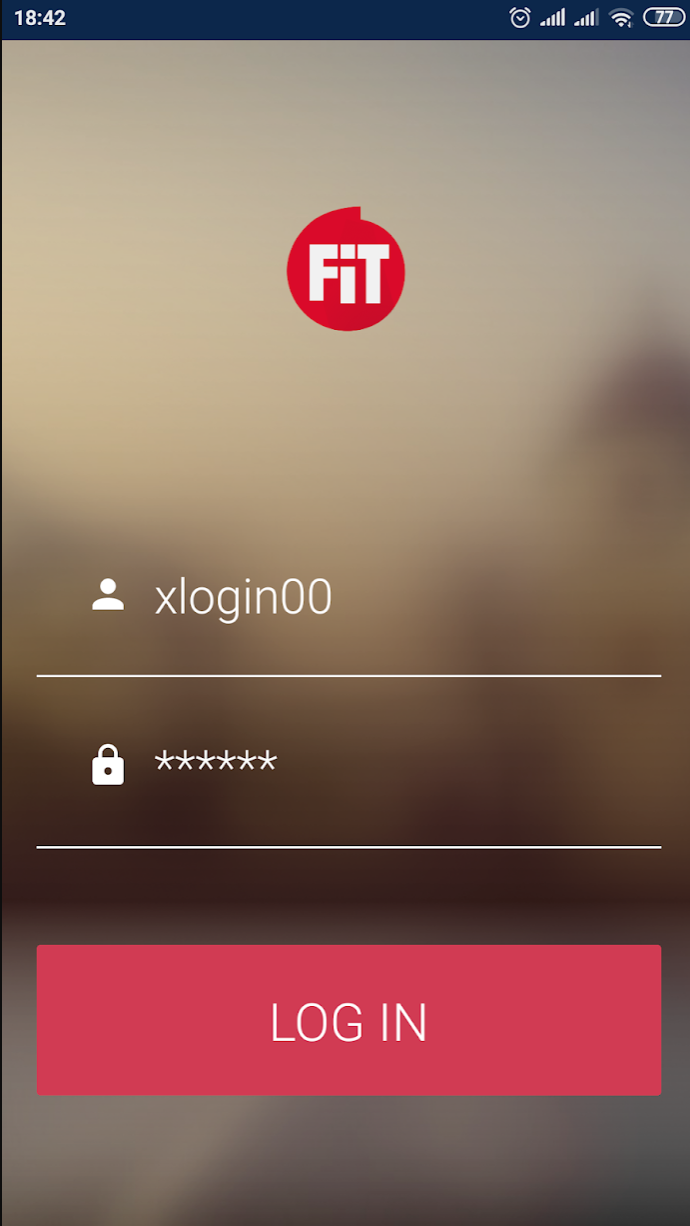
\includegraphics[width=.5 \linewidth, frame]{img/login.png}
		\caption{The login screen}
		\label{fig:activity-login}
	\end{subfigure}
	\begin{subfigure}{.48 \textwidth}
		\centering
		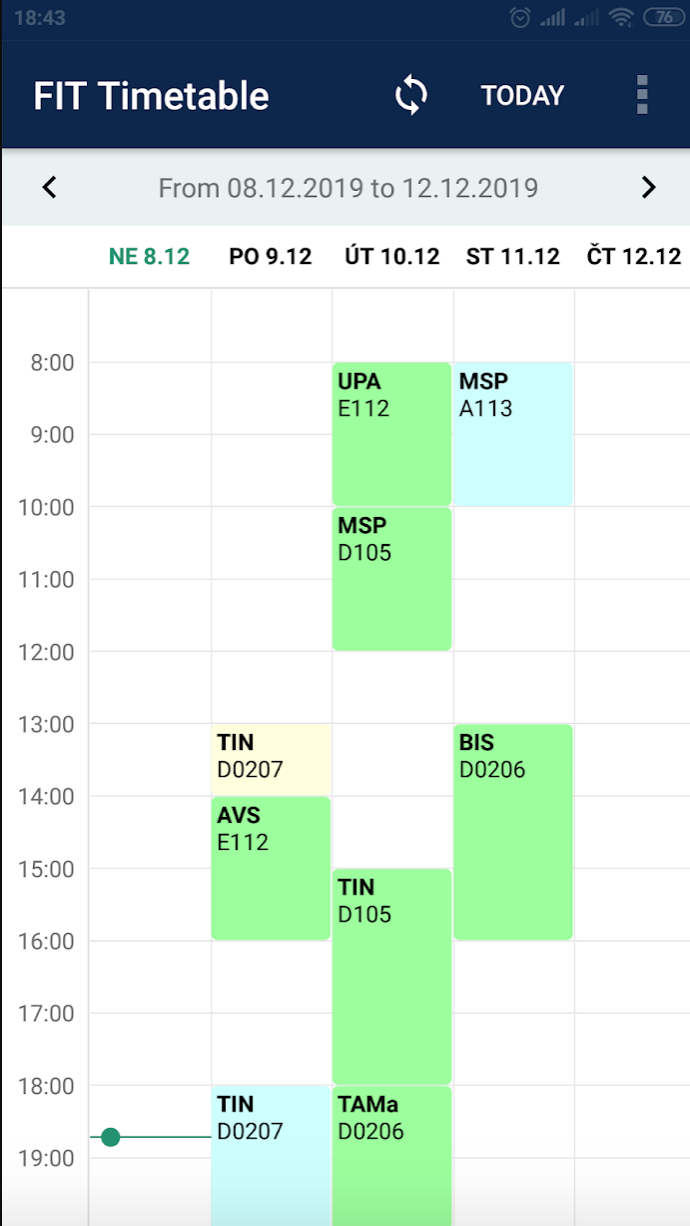
\includegraphics[width=.5 \linewidth, frame]{img/timetable.png}
		\caption{The main timetable screen}
		\label{fig:activity-timetable}
	\end{subfigure}

	\caption{The main screens of the application}
	\label{fig:main-activities}
\end{figure}

Furthermore, important achieved result is that we published the final
application on \emph{Google Play}, see Figure~\ref{fig:google-play}. Firstly,
we published it as a~beta version. And later, when we fixed some bugs, we
published it as a~stable version.

\begin{figure}[ht]
	\centering
	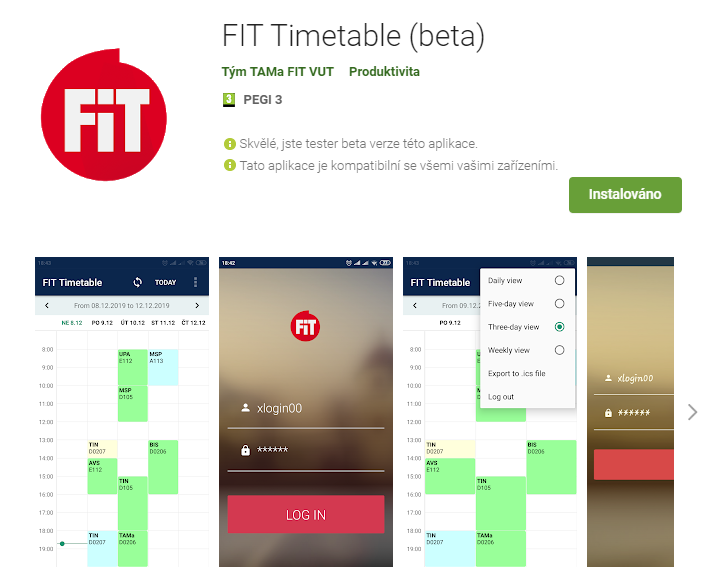
\includegraphics[width=.7 \linewidth, frame]{img/googleplay.png}
	\caption{The published application on Google Play}
	\label{fig:google-play}
\end{figure}

%-------------------------------------------------------------------------------

\section*{Controlling of Created Program}

Our application is very simple to use. To sign up it is necessary to fill in
a~login and a~password and press the \emph{Log in} button
(Figure~\ref{fig:activity-login}). After signing up, the application shows the
timetable for the actual week and weeks can be easily change by swiping the
screen or by tapping on arrows next to the date
(Figure~\ref{fig:activity-timetable}). Next, there is a~button for actualising
the timetable from the information system (it downloads a~current view of the
private timetable) and there is a~menu with several options such as:
\begin{itemize}
	\item daily view,
	\item three-day view,
	\item five-day view (default),
	\item weekly view, and
	\item export to \emph{.ics} file (for export to different applications).
\end{itemize}

%-------------------------------------------------------------------------------

\section*{Experience with the Selected Platform}

We were programming in \emph{Android Studio} using GitHub to share the code. As
new users of Android Studio, we were pleased to work with this tool\,--\,it helps
with syntax, orientation in a~code, downloading needed libraries, etc. To
simulate the code, we were using an emulator with different devices. We struggle
the most with logging to the information system using VUT and FIT certificates
(using \texttt{TrustManagerFactory}, \texttt{CertificateFactory}, SSL
context)\,---\,we could not find out how to write the certificate to the mobile
storage and how to read the context on a~device.

%-------------------------------------------------------------------------------

\section*{Distribution of the Work in the Team}

\begin{itemize}
	\item
		\textbf{Alena} designed and created a~user interface. She dealt with
		a~graphics framework. She also led the team. Finally, she linked
		frontend with the backend API.

	\item
		\textbf{Petr} created a~backend API for downloading and parsing
		the timetable from the FIT VUT information system into appropriate
		data structures. He also created an API for authenticating to that
		system.

	\item
		\textbf{Dominik} created a~feature that allows exporting timetable
		to different applications. He also tested the application and fixed
		some frontend bugs. At last, he deployed the application to the
		Google Play.
\end{itemize}

%-------------------------------------------------------------------------------

\section*{What Was the Biggest Challenge}

As it was already mentioned above, one of the biggest challenges was to manage
\emph{authenticating} to the FIT VUT information system because we had to work
with suitable \emph{certificates}. Quite time-consuming was \emph{parsing HTML
pages} from the information system because there is no documentation how these
pages could look like. Further, it was challenging to deal with the user
interface. In particular, it was not easy to create \emph{timetable view}. In
the end, we used a~framework for that.

%-------------------------------------------------------------------------------

\section*{Experience Gained From the Project}

We learned how to design a~user interface for mobile devices, particularly
for the latest Android devices. Furthermore, we learned how to use Android
Studio for Android development, we improved our Java skills, and we
learned the basics of Kotlin language. We also gained some experiences of
parsing HTML pages and using SSL certificates. Finally, we learned how
Android applications deployment works.

%-------------------------------------------------------------------------------

\section*{Autoevaluation}

\paragraph{Technical Design (95\,\%):}
At first, we created \emph{backend API} for authentication to the information
system and downloading and parsing timetable from that system. Then,
we designed and created a~user interface and we linked it with the backend
API. For the frontend timetable view, we selected appropriate framework.

\paragraph{Programming (80\,\%):}
We used the \emph{object-oriented paradigm}. The code is split into several
classes. Some classes are written in Java and some in Kotlin. Methods in
classes are sensible named so the overall code is quite readable. In run-time,
exceptions are caught and appropriate messages are shown to a~user.
The backend is general and it can be used in other applications as well.

\paragraph{Usability of the Created Solution (90\,\%):}
The application can be easily used by students of the FIT VUT. Some of the
students already installed and tried the application and they were
satisfied with it.

\paragraph{Use of Resources (70\,\%):}
We used the \emph{Android Week View} framework for displaying the timetable.
During the development process, we were using Android and Java documentation.
For downloading and parsing the timetable, we used handy Java libraries.

\paragraph{Time Management (75\,\%):}
In the beginning, we planned to implement more features and extensions but
finally, we did not have time for it. However, we implemented core
functionality on time and we had enough time for testing and fixing major
bugs.

\paragraph{Team Cooperation (90\,\%):}
We were seamlessly communicating via \emph{Messenger}. We split the work
between team members at the beginning of the semester and we also had several
personal meetings, primarily before project workshops.

\paragraph{Chances of Publishing the Application (100\,\%):}
The application is already published on Google Play. It is available on the
following link
\url{https://play.google.com/store/apps/details?id=com.tam.fittimetable}.

\paragraph{Overall Impression (80\,\%):}
The main goal was achieved. The application is useful for students of the
FIT VUT and it is published. Source codes are available on GitHub so it can
be extended in the future. We gained many useful skills and experience, as
it is described above.

%-------------------------------------------------------------------------------

\section*{Five Main Questions of TAM}

\paragraph{What drives this sector of IT? \\}

This sector of IT is driven by the \emph{increasing number of mobile phone
users}. More and more people own a~mobile phone and nowadays almost everyone
has one. People carry their phones always with them so they use them for
communicating, keeping notes, for entertainment, for paying, for controlling
their smart homes, etc.

\paragraph{What it will be like in five years? \\}

It will probably be more-less the same as nowadays. Of course, there will be
significantly more applications. Maybe, there will be new applications
related to \emph{virtual reality} and the \emph{internet of things}.

\paragraph{What slows it down, speeds it up? \\}

The factor that speeds it up is that there are more and more powerful devices
with \emph{efficient hardware}. In the other hand, currently, there are many
different versions of operating systems. Moreover, there are two
different widely used operating systems (iOS and Android). So this fact
slows this sector down.

\paragraph{What ideas are dead (though they appeared great once)? \\}

The \emph{Windows Phone operating system} is dead, although it had potential
and it was quite successful from the beginning. Another promising idea which
is now dead is a~\emph{hardware keyboard} on smartphones.

\paragraph{Where do new ideas come from? \\}

The most new ideas come from \emph{people's everyday demands and needs}. New
applications are based on ideas of how to make \emph{people's life easier}.

%-------------------------------------------------------------------------------

\section*{Recommendation for Assigning Future Projects}

The \emph{project workshops} are good. The acquired \emph{feedback} is often
very useful. It was also very nice that we had a~chance to pick
our \emph{own assignment} and even \emph{own platform}, so we could learn
exactly what we wanted to.

One disadvantage of this project that we have to mention is \emph{late
information} about when and how to send slides to project workshops.
These dates and instructions maybe can be available beforehand for the
whole semester.

%-------------------------------------------------------------------------------

\section*{Recommendation for Future Students}

In such a~project, think of a~\emph{really minimalist} and \emph{useful}
application and do it properly. Probably, you will be in time pressure and there
will not be enough time to finish your project. At the beginning of this
course, you might think that your selected assignment is simple and that
it will be easy to design and implement it. But try to truly \emph{think of
the problem}, its \emph{design}, and \emph{development}. Finally, pick something
\emph{simple} and focus on it from the beginning. Focus on design,
implementation, testing, and deployment.

%-------------------------------------------------------------------------------
\end{document}
